\documentclass{beamer}
\usecolortheme{orchid}
%\usepackage{graphicx}
\usepackage{hyperref}
\hypersetup{
    colorlinks=true,
    linkcolor=blue,
    filecolor=magenta,      
    urlcolor=cyan,
}
\usepackage[autoplay,loop]{animate} % I stuck the `autoplay' and `loop' functions up here to make it the default.

\title{Embedding ``GIFs'' in Beamer Slides \\ Memes for Fun, Profit, and Embarrassing Your Colleagues}
\author{Alton B.H. Worthington}
\institute{abhworthington.com}
\date{December 2016}

% This block of comment is to 1) Thank folks on Twitter for giving me something better to do on a couple of evenings than work on a dissertation 2) apologize to those who have seen this slide format before at a conference - I only have one style 3) apologize for my crummy code and lame jokes, and 4) disclaim all responsibility for all of that stuff that lawyers talk about at the end of pharmaceutical commercials.

% PS: I release all ownership of this LaTeX code. Use, splice, edit, distribute as you will. Credit would be nice, but ¯\_(ツ)_/¯.

\begin{document}
\beamertemplateshadingbackground{blue!10}{gray!30}
\usenavigationsymbolstemplate{}
\frame{\titlepage}

\begin{frame}
	\frametitle{A few quick notes}
	\begin{itemize}
		\item If you are viewing this on GitHub directly, please download it! (The images will not render/play properly in the GH viewer.)
	
		\item All of the animation fun to come does not work in some PDF viewers (OSX Preview and Foxit Reader are known-bad readers), but works well in the original Acrobat Reader and other readers which support Rich Media PDFs.
	
		\item If you're willing to try to put GIFs into a beamer presentation, this hiccup is likely minor.
	\end{itemize}
\end{frame}

\begin{frame}
	\frametitle{Motivation}
	Why even bother with GIFs? GIFs are:
		\begin{itemize}
			\item Super Old-school
			\item Space-inefficient (you want 400MB presentations? This is how you get 400MB presentations.)
			\item Not particularly attractive
			\item Actually kind of a pain in the butt to do in \LaTeX
			\item Guaranteed to be mentioned in your tenure file... I assume.
		\end{itemize}
	This seems like a bad idea. Are you sure?
\end{frame}

\begin{frame}
	\begin{center}
	\animategraphics[width=.75\linewidth]{25}{jack/jack-}{0}{82} %this command is: \animategraphics[options]{frames per second}{root of filename}{first frame number}{last frame number} - I knew to use 33.33 fps because I cheated and looked at the GIF properties (30ms per frame) in GIMP. You may choose to eyeball this. This all comes up again in the slides later on down there. Also, I stuck my gif frames in folders for safekeeping, hence the filename structure. The file name was "jack-0.png", for instance.
	\end{center}
\end{frame}

\begin{frame}
	\frametitle{I lied to you. That wasn't a GIF. (If you didn't notice already.)}
	Unfortunately, you can't really put a GIF directly into a PDF anymore. One used to be able to cram it into a PDF, open it in Acrobat Reader, then let an outboard player (like Flash Player) do the work. This is no longer an option. This is also, given the concerns on the previous slide, a ``good thing''.
	\begin{block}{I Made a Huge Mistake}
		Since I haven't tried to put a GIF in a slideshow in years, I never realized things had changed before I promised this instructional document. I lied. I'm sorry. Or, blame the PDF standard-setters. Your call.
	\end{block}
	The good news is that you can still ``embed'' a ``GIF'', but there's a bit more legwork to it. You still want to do this thing?
\end{frame}

\begin{frame}
	\frametitle{But I want to make bad career choices!!!!}
	Ok. Suit yourself.
	\begin{figure}
		\centering
		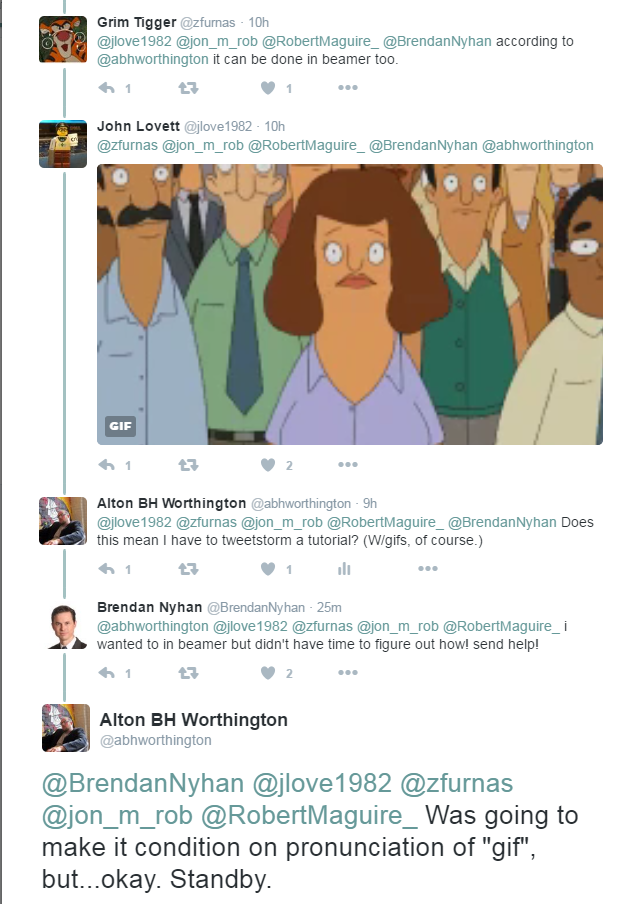
\includegraphics[scale=.25]{genesis.PNG}
	\end{figure}
	We all make mistakes. \pause I mean, I took the time to make a meta-beamer stack. If you're sure about this, proceed.
\end{frame}

\begin{frame}
	\frametitle{Ingredients}
	Congratulations! You've decided to make memetics a pedagogical strategy. Here's what you need:
		\begin{itemize}
			\item A gif. Or gifs.
			\item \href{https://www.imagemagick.org/script/binary-releases.php}{ImageMagick} or some other image converter.
			\item Beamer
			\item A bit of time and a folder to hold everything - your GIF is going to become a series of frames
			\item Optional, but recommended: \href{https://www.roosroast.com/}{coffee}
		\end{itemize}
	This is a beginner's guide, the ``hello world'' version of this process. I'll direct you to more documentation at the end of this stack. The process takes a few ``supersteps'', which I've broken down into smaller steps.
\end{frame}

\begin{frame}
	\frametitle{Step 1a: Acquire the Memes of Production}
	This should be self explanatory. Find a gif you like or which is relevant to your interests. Good candidates include:
		\begin{itemize}
			\item Cats
			\item Movies
			\item Famous people
			\item Relatable cartoons
			\item Internet esoterica
		\end{itemize}
	Shorter GIFs work better for this, but it's not a huge deal.
\end{frame}

\begin{frame}
	\frametitle{Step 1b: Premium GIFs}
	If you can get multiple at once, you're in with a shot at a conference award. (Please share the award money.)
	\begin{center}
	\animategraphics[width=\linewidth]{18}{cat/cat-}{0}{49}
	\end{center}
	\end{frame}

\begin{frame}
	\frametitle{Step 1c: Saving and Organizing}
	Once you've found your premium GIF material:
		\begin{enumerate}
			\item Create a folder somewhere convenient. (read: somewhere with a short filepath)
			\item Save the GIF to that convenient location.
			\item Prepare to break your GIF up.
		\end{enumerate}
\end{frame}

\begin{frame}
	\frametitle{Step 2a: Breaking Up}
	GIFs are great, but they won't work as-is in beamer or in \LaTeX. You could convert it to a movie, but an easier route  is to create images and animate it. You've got a few options:
		\begin{itemize}
			\item Various web services (that's between you and Google)
			\item GIMP or other image editing software
			\item or, my recommendation: \href{https://www.imagemagick.org/script/binary-releases.php}{ImageMagick}
		\end{itemize}
	ImageMagick has a bit of a learning curve, but let's face it: You're using \LaTeX. You've got this. \hyperlink{STEP3a}{If you want to use some other sort of program to create your image stack, click here and you'll rejoin us after the ImageMagick bits.}
\end{frame}

\begin{frame}
	\frametitle{Step 2b: Download and Install ImageMagick}
	I use ImageMagick to convert a GIF into individual images. It does \emph{a whole lot more}, but for today, we are just going to use it to convert the GIF into a stack of PNG images, which pdflatex finds easy to digest. First you have to download and install it! \\
		\begin{itemize}
			\item In Windows, \href{https://www.imagemagick.org/script/binary-releases.php\#windows}{download and execute this installer}.
			\item If you are using any Linux/Unix, \href{https://www.imagemagick.org/script/binary-releases.php\#unix}{you can get a binary here}.
			\item In OSX, things are a bit complicated. The easiest way is to install ImageMagick via HomeBrew. \href{https://github.com/abhworthington/gifsinbeamer/blob/master/ImageMagickscripts/OSX/OSXfirsttime.txt}{Follow the instructions (for both) I've written here}.
		\end{itemize}
	The next step is the only bit of command line messiness you need to deal with. Sorry. It's worth it, I promise. But first, an ``out''.
\end{frame}

\begin{frame}
	\frametitle{Step 2c: From GIF to PNG}
	If you want to do this the easiest way, I've put scripts on GitHub for your use.
	\begin{itemize}
		\item The Windows executable batch file is here: \href{https://raw.githubusercontent.com/abhworthington/gifsinbeamer/master/ImageMagickscripts/giftopng.bat}{Right-click and save as a .bat file.} (This may require deleting a suffix.)
		\item If you use OSX, that script is here. \href{https://github.com/abhworthington/gifsinbeamer/blob/master/ImageMagickscripts/giftopng.command}{Save the file as a .command file.} You'll also need to change permissions on the script. \href{https://github.com/abhworthington/gifsinbeamer/blob/master/ImageMagickscripts/OSX/OSXfirsttime.txt}{I explain how to do that here}.
	\end{itemize}
	The script should be placed in the same folder as \emph{one GIF only}. This is important. The script creates an output folder and drops the frames inside. Then you can just take them away to where you need them. \hyperlink{STEP3a}{If you use the scripts, you can click here.} If you want to DIY, continue.
\end{frame}

\begin{frame}[fragile]
	\frametitle{Step 2d: Command Line Work}
	If you want to run the command yourself, open a command window and run:
		\begin{block}{For Windows 7/8/10}
		\begin{verbatim}
		magick "*.gif" -coalesce "gifoutput\gifoutput.png"
		\end{verbatim}
		\end{block}
	Here, ``*.gif'' is the input file and ``gifoutput.png'' is the root of the output filenames. I created a folder to hold them in the batch script called ``gifoutput''. The ``-coalesce'' option before the output ensures full frames, not partial ones of different size, are created. (There's a lot more you can do, but I leave the ImageMagick documentation to the reader.)
\end{frame}

\begin{frame}[fragile]
	\frametitle{Step 2d: Command Line Work}
	If you want to run the command yourself, open a terminal and run:
		\begin{block}{For OSX}
		\begin{verbatim}
		convert *.gif -coalesce gifoutput.png
		\end{verbatim}
		\end{block}
		Here, *.gif is the input file and gifoutput.png is the root of the output filenames. You can append paths as needed. The ``-coalesce'' option before the output ensures full frames, not partial ones of different size, are created. (There's a lot more you can do, but I leave the ImageMagick documentation to the reader.)
\end{frame}

\begin{frame}\hypertarget{STEP3a}{}
	\frametitle{Step 3a: Animating in Beamer}
	Now that you have a stack of images (I like PNG for this), you are almost ready to go. But first:
	\begin{block}{One important notice!!!}
		Your images have to have a consistent naming scheme, with numbers at the end. This means something like ``jack-0.png'', then ``jack-1.png'', etc. on until the last frame. For the nodding Jack Nicholson above, it was ``jack-0.png'' up to ``jack-82.png''. If your frames are not numbered, you are gonna have a bad time. You have to put them somewhere your \TeX editor can find them.
	\end{block}
	Now I'll introduce you to the reason for this whole endeavor - the ``animate'' package. (It's great, and has value well beyond the simple meme.)
\end{frame}

\begin{frame}[fragile]
	\frametitle{Step 3b: Using \emph{animate} to... animate.}
	Putting animations in your presentation (or document, if so inclined) is really complicated. (\textbackslash s)
		\begin{itemize}
			\item Use \verb+\usepackage{animate}+ in the preamble
			\item Use \verb+\animategraphics+ in your frames/text
		\end{itemize}
	Each of these requires a quick primer, but once you do it once, it becomes trivial to do.
\end{frame}

\begin{frame}[fragile]
	\frametitle{Step 3c: The animate Preamble}
	You can call the ``animate'' package as it is, but if you intend to put several animations in your slide deck, you can save yourself time and energy by putting some commands in the preamble call. The full call is: \verb+\usepackage[options]{animate}+. Some useful options are:
		\begin{itemize}
			\item autoplay - when the page is up, the animation starts
			\item loop - the animation goes from first frame to last, then repeats
			\item controls - puts basic controls on the image stack
			\item autopause - pauses, rather than resets, when you leave the page
			\item palindrome - first to last to first play
			\item step - one click per frame (this will make sense in a second)
		\end{itemize}
	I tend to drop \verb+[autoplay, loop]+ in my options every time, including here. Comma separate!
\end{frame}

\begin{frame}[fragile]
	\frametitle{Step 3d: The `animategraphics' command}
	The last step is actually including the image. As long as you did your prep work right, this is easy. The full command is:
		\begin{block}{The Magic Command}
			\begin{verbatim}
			\animategraphics[options]{frames per second}
			{filename w/o number or suffix}{start #}{end #}
			\end{verbatim}
		\end{block}
		\begin{block}{An example}
			\begin{verbatim}
			\animategraphics[width=\linewidth]{25}{jack-}{0}{82}
			\end{verbatim}
			The filenames were ``jack-0.png'' to ``jack-82.png''. I set width to the textbox width and ran the animation at 25 fps.
		\end{block}
\end{frame}

\begin{frame}
	\frametitle{Step 3e: Framerate and Size}
	Sizing works the same as the ``graphics'' commands, but framerate may be new to you. Here's a gif at ``proper'' speed - 10 fps.
		\begin{center}
		\animategraphics[width=\linewidth]{10}{steve/steve-}{0}{26}
		\end{center}
\end{frame}

\begin{frame}
	\frametitle{Step 3e: Framerate and Size}
	Here's the same gif at double speed - 20 fps.
		\begin{center}
		\animategraphics[width=\linewidth]{20}{steve/steve-}{0}{26}
		\end{center}
	Have fun with this.
\end{frame}

\begin{frame}
	\frametitle{Step 4: There is no ``Step 4''}
	You're done. Bask in the glow of a job well done. Enjoy the applause at your next presentation. Please use in moderation. You can also use this to great effect with other graphics, like plots where time (or another dimension) is relevant. Try it! If you want to see a couple more tricks and references, continue.
\end{frame}

\begin{frame}
	\frametitle{If all has gone well, you'll look at your presentations like:}
	\begin{center}
	\animategraphics[width=\linewidth]{20}{comp/comp-}{0}{223}
	\end{center}
\end{frame}

\begin{frame}
	\frametitle{Your presentations are gonna be so great, your audience will:}
	\begin{center}
	\animategraphics[width=\linewidth]{12.5}{lakerbros/lakerbros-}{0}{42}
	\end{center}
\end{frame}

\begin{frame}
	\frametitle{Or, better yet:}
	\begin{center}
	\animategraphics[width=\linewidth]{12.5}{lakerbros/lakerbros-}{42}{0}
	\end{center}
	\pause
(Those are the same files, btw. Just reversed the frame order. \{0\}\{42\} becomes \{42\}\{0\}. Try it. It's fun.)
\end{frame}

\begin{frame}
	\frametitle{References/Additional Info}
	
		\begin{itemize}
			\item \href{https://www.imagemagick.org/script/index.php}{ImageMagick} 
			\item \href{http://tug.ctan.org/macros/latex/contrib/animate/animate.pdf}{The `animate' package reference doc}
			\item \href{http://tug.ctan.org/macros/latex/contrib/beamer/doc/beameruserguide.pdf}{The `Beamer' class User Guide}
		\end{itemize}
	
\end{frame}

\begin{frame}
	\frametitle{Thanks to:}
	\begin{itemize}
		\item Till Tantau, Joseph Wright, and Verdan Mileti\'{c} (Beamer)
		\item Alexander Grahn (animate)
		\item Zander Furnas, Brendan Nyhan, Jonathan Robinson, and John Lovett, for requesting (and waiting patiently for) this document.
		\item Matt Malesky, for help with the OSX shell file process.
		\item Erin Cikanek, for being a patient OSX workflow beta-tester.
	\end{itemize}
	And, of course, thanks to the massive community at \href{http://stackoverflow.com/}{Stack Overflow}, who explained this already in a different question.
\end{frame}

\end{document}